% !TEX root = SegwayDoku.tex
\renewcommand{\autoren}{Valentyn Chepil}
\newpage
\section{Die Hindernis umfahren}

Die benötigten, reaktiven Fähigkeiten ”Hindernis umfahren”, (bzw. ”Hindernis rechts umfahren” und ”Hindernis links umfahren”) können alternativ mithilfe der Regelungstechnik und zweier grundlegender Teilschritte realisiert werden. Der prinzipielle Ablauf der reaktiven Fähigkeit ist in Abbildung \ref{bild_HUR} dargestellt. 

\begin{figure}[!h]  % [h] bedeutet, dass das Bild genau an dieser Stelle im Text erscheint
	\centering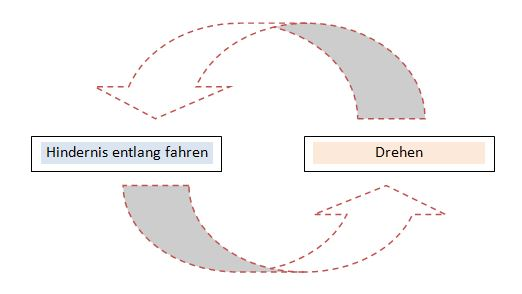
\includegraphics[width=0.6\textwidth]{images/Bild_HUR.jpg}
	\caption{ \ Regelkreis "Hindernis umfahren" (Quelle:Eigene Darstellung)}
	\label{bild_HUR} % über das label kann man aus dem Text auf das Bild verweisen
\end{figure}

In der Abbildung sind zwei prinzipielle Teilschritte abgebildet und durch zwei Farben gekennzeichnet. Zuerst soll sich der Glied in Bezug auf das Hindernis richtig ausrichten, siehe Teilschritt ”Drehen”, anschließend entlang des Hindernisses fahren. Diese beiden Teilschritte werden noch weiter unterteilt. Der Schritt Drehen wird je nach vorgegebener Richtung in ”Drehen rechts” und ”Drehen links” aufgeteilt. Dieser Teilschritt wird als vorgegebene Konstante realisiert. ”Hindernis entlang fahren” wird in die Teilschritte ”Hindernis rechts entlang fahren” und ”Hindernis links entlang fahren” aufgeteilt und mithilfe der PID-Regler realisiert. 

\begin{figure}[!h]  % [h] bedeutet, dass das Bild genau an dieser Stelle im Text erscheint
	\centering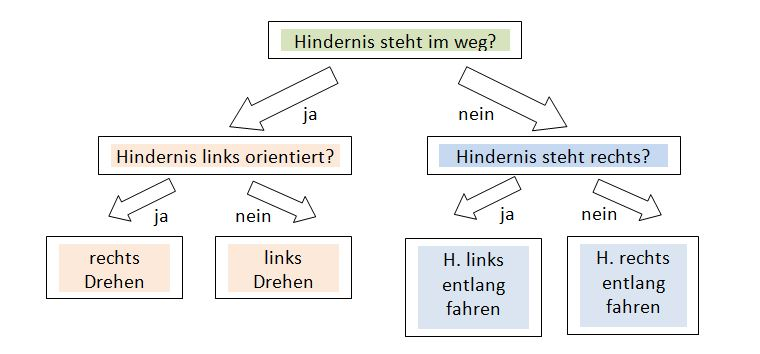
\includegraphics[width=0.8\textwidth]{images/Entsch_baum.jpg}
	\caption{ \ Entscheidungsbaum für "Hindernis umfahren" (Quelle:Eigene Darstellung)}
	\label{baum} % über das label kann man aus dem Text auf das Bild verweisen
\end{figure}

 In diesem Fall wird in Abhängigkeit von der aktuellen Orientierung des Hindernis entschieden, wie es am günstigsten ist sich zu drehen, um die Fahrt entlang des Hindernisses fortzusetzen.



%\subsection{PID-Regler}

%Der PID-Regler besteht aus den Anteilen des P-Gliedes, des I-Gliedes und des D-Gliedes. Er kann sowohl aus der Parallelstruktur oder der Reihenstruktur definiert werden.

%\begin{figure}[!h]  % [h] bedeutet, dass das Bild genau an dieser Stelle im Text erscheint
%	\centering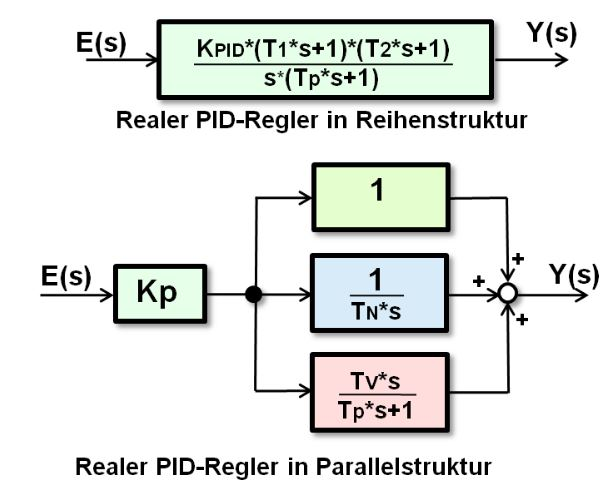
\includegraphics[width=0.6\textwidth]{images/PID.jpg}
%	\caption{ \ PID-Regeler (Quelle:Wikipedia)}
%	\label{pid} % über das label kann man aus dem Text auf das Bild verweisen
%\end{figure}

%Beide Darstellungsformen der parallel- und reihenstrukturierten PID-Regler, die sich mathematisch völlig identisch umrechnen lassen, haben unterschiedliche Vorteile in der Anwendung:

%- Die Reihenstruktur des PID-Reglers und die zugehörige Übertragungsfunktion erlauben für den Reglerentwurf die einfache Pol-Nullstellen-Kompensation von Regler und Regelstrecke.
 
%- Die Parallelstruktur des PID-Reglers ermöglicht das Verhindern des Wind-up-Effekts. Sehr häufig wird die Stellgröße des Reglers u(t) in Regelkreisen durch die Regelstrecke begrenzt. Dadurch entsteht das ungewollte Verhalten des I-Gliedes, bis zu seiner eigenen Begrenzung weiter zu integrieren. Verschwindet die Stellgrößenbegrenzung, weil die Regelabweichung gegen Null läuft, hat das I-Glied einen zu hohen Wert und verursacht eine schlechte Einschwingdynamik der Regelgröße y(t). 

%\textbf{Software Darstellung:} 

%esum = esum + e

%y = Kp * e + Ki * Ta * esum + Kd * (e – ealt)/Ta

%ealt = e
%
%\textbf{Mit:}  Kp-Proportionalbeiwert, Ki-Integralbeiwert, Kd-Differenzialbeiwert, e-Regelabweichung, Ta-Zeitkonstante.

% für Weiterinfo link:http://rn-wissen.de/wiki/index.php?title=Regelungstechnik

%\subsection{}

%\pagebreak
